% ============================================================================
% Deliverable 1 - Generative Artificial Intelligence (580694), Spring 2026
% Universidad de Concepcion
% Single-page poster / executive summary.
% Compile:  pdflatex deliverable1.tex   (run twice)
% ============================================================================
\documentclass[9pt,a4paper]{extarticle}

\usepackage[utf8]{inputenc}
\usepackage[T1]{fontenc}
\usepackage[margin=0.85cm,top=0.7cm,bottom=0.45cm]{geometry}
\usepackage{helvet}\renewcommand{\familydefault}{\sfdefault}
\usepackage{xcolor}
\usepackage{multicol}
\usepackage{booktabs}
\usepackage{enumitem}
\usepackage{tcolorbox}
\usepackage{pgfplots}
\usepackage{microtype}
\pgfplotsset{compat=1.16}
\tcbuselibrary{skins}

% ---------------------------------------------------------------- palette --
\definecolor{navy}{HTML}{16314F}
\definecolor{steel}{HTML}{3C5A80}
\definecolor{amber}{HTML}{B45309}
\definecolor{crimson}{HTML}{9B1C1C}
\definecolor{paper}{HTML}{F4F6F9}
\definecolor{rule}{HTML}{C9D2DE}
\definecolor{note}{HTML}{FDF3D8}

\setlength{\parindent}{0pt}
\setlength{\columnsep}{6.5mm}
\setlength{\multicolsep}{2pt}
\setlength{\parskip}{0.62mm}
\setlength{\intextsep}{1mm}
\pagestyle{empty}

% ---------------------------------------------------------------- helpers --
\newcommand{\heading}[1]{%
  \par\vspace{1.4mm}\noindent
  {\color{navy}\bfseries\small\MakeUppercase{#1}}
  \par\vspace{0.7mm}\noindent
  {\color{amber}\rule{\linewidth}{1.1pt}}
  \par\vspace{0.6mm}\noindent\ignorespaces}

\newtcolorbox{keybox}[1]{colback=note,colframe=amber,boxrule=0.8pt,
  left=2mm,right=2mm,top=1.5mm,bottom=1.5mm,arc=1mm,
  fonttitle=\bfseries\footnotesize,coltitle=white,colbacktitle=amber,title={#1}}

\newtcolorbox{quietbox}{colback=paper,colframe=rule,boxrule=0.5pt,
  left=2mm,right=2mm,top=1.5mm,bottom=1.5mm,arc=1mm}

\newcommand{\ph}[1]{\colorbox{yellow!60}{\textcolor{black}{\textbf{#1}}}}
\setlist[itemize]{leftmargin=3.6mm,itemsep=0.6mm,topsep=0.8mm,parsep=0pt}

\begin{document}
\small

% ================================================================== HEADER ==
\begin{tcolorbox}[colback=navy,colframe=navy,boxrule=0pt,left=3mm,right=3mm,
                  top=2mm,bottom=2mm,arc=1mm]
{\color{white}\bfseries\LARGE Small Language Models for Battle Decision-Making in Pok\'emon Blue}\\[1.1mm]
{\color{white!85}\large Structured prompting fixes action formatting, but not decision quality}\\[2mm]
{\color{white!75}\footnotesize
Deliverable 1 \ \textbullet\ \ Generative Artificial Intelligence (580694), Spring 2026 \ \textbullet\ \ Universidad de Concepci\'on}\\[1.4mm]
{\footnotesize\color{white!85}Team:} \ph{Nombre 1 \textbullet\ Nombre 2 \textbullet\ Nombre 3 \textbullet\ Nombre 4}
\hfill
{\footnotesize\color{white!85}Repository:} \ph{github.com/usuario/repositorio}
\end{tcolorbox}

\vspace{1.5mm}
\begin{multicols}{2}

% ============================================================ 1. THE TASK ==
\heading{1. Task specification}
The model acts as the \textbf{battle-decision module} of a Pok\'emon Blue agent.

\textbf{Input.} A structured battle state: both Pok\'emon's type(s), HP\%\ and Speed, plus the four available moves with \emph{name, type, power, accuracy} and \emph{remaining PP}.

\textbf{Output.} Exactly one executable label: \texttt{MOVE\_1}, \texttt{MOVE\_2}, \texttt{MOVE\_3} or \texttt{MOVE\_4}.

\textbf{What counts as correct.} The label that maximises an explicit, deterministic offensive policy,
\par\vspace{0.6mm}\noindent\hspace*{\fill}%
\colorbox{paper}{\;\texttt{score = power $\times$ accuracy $\times$ STAB $\times$ type-effectiveness}\;}%
\hspace*{\fill}\par\vspace{0.8mm}\noindent
with \texttt{score = 0} when \texttt{PP = 0}. The ground truth is therefore reproducible and auditable case by case.

\textbf{Why it is non-trivial.} The five attributes trade off: the highest-\emph{power} move is optimal in only 19 of 30 states, and Gen~I immunities (Electric\,$\to$\,Ground, Normal\,$\to$\,Ghost) zero out the strongest-looking option. The model must \emph{combine} constraints, not retrieve a fact.

% ======================================================= 2. PILOT SETUP ====
\heading{2. Pilot experiment (v1)}
\textbf{Model.} Qwen2.5-1.5B-Instruct, greedy decoding, \texttt{max\_new\_tokens=48}, seed \texttt{20260830}, identical system prompt in both conditions.

\textbf{Design.} 30 synthetic battle states (10 EASY / 10 MEDIUM / 10 HARD, graded by the best-vs-second score ratio: $\geq$1.80 / 1.25--1.80 / 1.01--1.25). \textbf{The same 30 states} go to both prompts $\rightarrow$ \textbf{60 inferences}, offline, with no emulator inside the measurement loop.

\textbf{Conditions.} \textsc{Direct} = natural request (``What move would you use next?''). \textsc{Structured} = same state, explicit reasoning checklist, and a hard output contract (\texttt{MOVE\_N} only).

\textbf{Metrics.} \textsc{Strict} (exactly \texttt{MOVE\_N}, executable) $\cdot$ \textsc{Interp} (intent recoverable) $\cdot$ \textsc{Acc} (matches ground truth) $\cdot$ \emph{regret} (share of the best score lost).

\vspace{0.8mm}
{\centering
\begin{tabular}{@{}lrrrr@{}}
\toprule
\textbf{Prompt} & \textsc{Strict} & \textsc{Interp} & \textsc{Acc} & \textsc{Exec-c.}\\
\midrule
\textsc{Direct}     & 0.0\%  & 36.7\% & 3.3\%  & 0.0\%\\
\textsc{Structured} & \textbf{96.7\%} & \textbf{96.7\%} & \textcolor{crimson}{\textbf{16.7\%}} & 16.7\%\\
\bottomrule
\end{tabular}\par}
\vspace{0.4mm}
{\footnotesize Mean regret: \textsc{Direct} 0.41, \textsc{Structured} 0.49. $n=30$ states per condition.}

% ==================================================== 3. FAILURE DIAGNOSIS ==
\heading{3. Failure diagnosis}
Structured prompting almost eliminated the \emph{interface} problem (\textsc{Strict} $0\%\rightarrow96.7\%$; one answer was still unexecutable), so the agent can now be driven automatically. It did \emph{not} solve the task --- decision quality stays \textbf{below chance}.

\textbf{The model answers by position, not by state.} Across the 29 parseable structured answers it returns \texttt{MOVE\_2} 20 times and \texttt{MOVE\_1} \emph{never}, while the optimal action is nearly uniform over the four slots ($\chi^2(3)=31.8$, $p<10^{-6}$ for its choice distribution against uniform).

\vspace{0.5mm}
{\centering
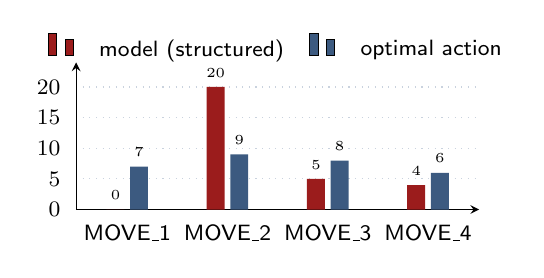
\begin{tikzpicture}
\begin{axis}[
  width=6.7cm, height=3.45cm, ybar, bar width=6.5pt,
  ymin=0, ymax=24,
  symbolic x coords={MOVE\_1,MOVE\_2,MOVE\_3,MOVE\_4},
  xtick=data, xticklabel style={font=\footnotesize},
  yticklabel style={font=\footnotesize}, ytick={0,5,10,15,20},
  legend style={font=\footnotesize,at={(0.5,1.24)},anchor=north,legend columns=2,
                draw=none,fill=none,column sep=2.5mm},
  axis lines=left, tick style={draw=none},
  ymajorgrids, grid style={rule,dotted},
  enlarge x limits=0.17, nodes near coords,
  every node near coord/.append style={font=\tiny}]
\addplot[fill=crimson,draw=none] coordinates {(MOVE\_1,0)(MOVE\_2,20)(MOVE\_3,5)(MOVE\_4,4)};
\addplot[fill=steel,draw=none]   coordinates {(MOVE\_1,7)(MOVE\_2,9)(MOVE\_3,8)(MOVE\_4,6)};
\legend{model (structured), optimal action}
\end{axis}
\end{tikzpicture}\par}
\vspace{-0.5mm}

\textbf{It only scores when the answer happens to be \texttt{MOVE\_2}.} Hit rate by the position of the optimal move: \texttt{MOVE\_1} \textbf{0/7}, \texttt{MOVE\_2} 4/9, \texttt{MOVE\_3} 1/8, \texttt{MOVE\_4} \textbf{0/6}.

\textbf{Trivial policies beat the model.}
\vspace{0.8mm}

{\centering
\begin{tabular}{@{}lr@{}}
\toprule
\textbf{Policy} & \textbf{Accuracy}\\
\midrule
Qwen2.5-1.5B, structured prompt   & \textcolor{crimson}{\textbf{16.7\%}}\\
Uniform random over 4 moves       & 25.0\%\\
Constant ``always \texttt{MOVE\_2}'' & 30.0\%\\
$\max$(power $\times$ accuracy), PP\,$>$\,0 & 53.3\%\\
$\max$(power) --- ignores types entirely & \textbf{63.3\%}\\
\bottomrule
\end{tabular}\par}
\vspace{1.4mm}

\begin{keybox}{Diagnosis}
The main observed bottleneck is \textbf{not} output formatting but \textbf{multi-constraint action selection}: asked to weigh type effectiveness, STAB, power, accuracy and PP over four candidates at once, the 1.5B model collapses onto a \textbf{position prior} that is almost independent of the battle state. A one-line heuristic that ignores type charts altogether is \textbf{3.8$\times$} more accurate.
\end{keybox}

% =================================================== 4. VALIDITY CHECKS =====
\heading{4. Is the ground truth the problem?}
A low score against a hand-made policy could just mean the policy is wrong. Three checks say otherwise --- these errors are indefensible under \emph{any} rule:
\begin{itemize}
\item \textbf{Zero-effect move.} Case 16 (below): \emph{Thunderbolt} (Electric) into a \textbf{Ground} opponent --- immune, 0 damage.
\item \textbf{Unexecutable move.} Case 29: a move with \textbf{PP = 0}; the agent physically cannot issue it.
\item \textbf{Strictly worst option} chosen in \textbf{6 of 29} answers (21\%) --- the lowest-scoring of the four.
\end{itemize}

\vspace{-0.5mm}
\begin{quietbox}
{\footnotesize\ttfamily
CASE 16 -- player Flying (41\% HP) vs Ground (53\%)\\[0.4mm]
MOVE\_1 Psybeam\ \ \ \ Psychic\ \ P65 A100 \ \ score 65.0\\
MOVE\_2 Thunderbolt Electric P95 A100 \ \ score \ \textcolor{crimson}{\textbf{0.0}}\\
MOVE\_3 Rock Throw\ \ Rock\ \ \ \ \ P50 \ A65 \ \ score 16.3\\
MOVE\_4 Ember\ \ \ \ \ \ Fire\ \ \ \ \ P40 A100 \ \ score 40.0\\[0.6mm]
ground truth = MOVE\_1 \ \ \ \ model = \textcolor{crimson}{\textbf{MOVE\_2}}}\\[0.6mm]
{\footnotesize The model takes the highest \emph{power} number and ignores the immunity that makes it useless.}
\end{quietbox}

\textbf{No difficulty gradient.} Structured accuracy is EASY 2/10, MEDIUM 1/10, HARD 2/10. Graded reasoning should degrade as cases get harder; a position prior should not --- and it does not.

% ======================================================= 5. THREATS + V2 ===
\heading{5. Threats to validity, and the v2 fix}
\begin{itemize}
\item \textbf{T1.} \textsc{Direct} never requested \texttt{MOVE\_N}, so its $0\%$ \textsc{Strict} is true by construction; it is reported as an \emph{interface baseline}, not as reasoning evidence.
\item \textbf{T2.} \texttt{max\_new\_tokens=48} truncated free-text \textsc{Direct} answers, deflating its 36.7\% \textsc{Interp}.
\item \textbf{T3.} The reference policy is offensive-only: no status moves, switching, items or multi-turn play.
\end{itemize}
\textbf{v2.} Both prompts enforce the same \texttt{MOVE\_N} contract, so the only difference is the reasoning scaffold; $n=50$ states; every state replayed with its moves \textbf{permuted}, measuring the position prior directly.

% ==================================================== 6. MODEL CANDIDATES ==
\heading{6. Proposed models (all far below 8B)}
{\centering
\begin{tabular}{@{}lrrrrr@{}}
\toprule
\textbf{Model} & \textbf{Par.} & \textbf{MMLU} & \textbf{IFEval} & \textbf{GSM8K} & \textbf{fp16}\\
\midrule
Qwen2.5-1.5B-Instr. & 1.5B & 50.7 & 42.5 & 73.2 & 3.1\,GB\\
Llama-3.2-3B-Instr. & 3.2B & 63.4 & \textbf{77.4} & 77.7 & 6.4\,GB\\
Phi-3.5-mini-instr. & 3.8B & \textbf{69.0} & n.r. & \textbf{86.2} & 7.6\,GB\\
\bottomrule
\end{tabular}\par}
\vspace{0.3mm}
{\footnotesize Sources: official model cards for Qwen2.5, Llama 3.2 and Phi-3.5-mini (full references in the repository). Protocols differ, so the figures place the models in a class rather than rank them. n.r. = not reported.}
\vspace{0.6mm}

\begin{itemize}
\item \textbf{IFEval: instruction following.} A general benchmark for obeying constrained output formats, which is what the controller needs. Note that under the structured prompt Qwen already reaches 96.7\% compliance despite its 42.5, so format is \emph{not} what separates the candidates.
\item \textbf{GSM8K: multi-step reasoning.} The closest public proxy to the step that does fail here, combining several numeric attributes. Phi-3.5-mini leads at \textbf{86.2} with only 3.8B: the direct test of whether that bottleneck lifts.
\end{itemize}
Qwen2.5-1.5B is also the baseline: the only candidate with a \emph{measured} profile on this task. The task does not obviously require an 8B model, which motivates evaluating substantially smaller candidates; the largest here is \textbf{3.8B}.

\end{multicols}

\vspace{-2mm}
\begin{tcolorbox}[colback=paper,colframe=navy,boxrule=0.9pt,left=2.5mm,right=2.5mm,
                  top=1.4mm,bottom=1.4mm,arc=1mm,
                  fonttitle=\bfseries\footnotesize,coltitle=white,colbacktitle=navy,
                  title={7. EXECUTION FEASIBILITY \& REPRODUCIBILITY}]
\footnotesize
The pilot \textbf{already ran end to end} on the team's own hardware: 60 inferences, \textbf{105.5 min} wall-clock on \textbf{CPU}, deterministic (greedy, fixed seed). Memory estimated as parameters $\times$ 2 bytes (fp16) plus KV cache: all three fit in a free Colab T4 (16\,GB), and Qwen2.5-1.5B is verified directly by the pilot. The repository ships the benchmark script, its four result artefacts and the PyBoy demo --- kept \emph{outside} the measurement loop, so emulator-control bugs can never be mistaken for model failures. \hfill \mbox{\textbf{Repo:} \ph{github.com/usuario/repositorio}}
\end{tcolorbox}
\end{document}
